\subsubsection{Langeweile} \label{langeweile-4}


In diesem Prototyp wird nur das ``Pec-Turning'' Spiel als Szenario benutzt, da die Zeit des Experiments reduziert werden sollte. Allerdings gib es ein kleines Unterschied mit dem Spiel von dem ersten Prototyp. 
Hier wird die grüne kreisförmige Scheibe nicht mehr durch ein Mausklick, sondern durch den Controller von der VR  in Bewegung gebracht. Nach jeder Bewegung des Kreis muss man mindesten fünften Sekunde warten bis die nächste Bewegung möglich ist.
Um dies Szenario in Unreal Engine zu verwirklichen wurde erst mal ein Widget Blueprint erstellt. 
Dann wurde vier mal das Bild von dem Spiel genau an der gleiche Stelle und in der gleiche Große in der Widget hinzugefügt. 
Das erste Bild sollte in der Ausgangsposition sein. 
Dann sollte jedes der nächsten Bilder eine Drehung des vorherigen Bildes um neunzig Grad sein. 
Es sollte von Anfang an das Ausgangsbild auf sichtbar gesetzt und die anderen auf unsichtbar. 
Danach wurde einen transparenten Button immer auf die Bilder der Scheiben eingefügt, um das Wechsel von Bilder zu steuern. 
Zur Programmierung wurde eine Funktion mit Timeout und Branch-Bedingung erstellt und der Algorithmus wurde so rekursiv definiert: 
Wenn das Button gedrückt ist, wird das nächste Bild auf sichtbar (``visible'') gesetzt und die anderen Bilder auf unsichtbar (``invisible''), dann wird ein Timeout gesetzt und eine Branch-Bedingung soll Prüfen ob das Timeout durch ist. Sollte vor dem Ende des Timeouts der Button gedrückt werden, so sollte nichts passieren. 
Wenn das Timeout fertig ist, soll das Szenario sich wiederholen. 
Es wird auch jede zeit durch einen Text in einem Textfeld gezeigt, wenn man die Scheibe drehen kann und wenn man warten muss. 
Ein letztes Timeout wurde hinzugefügt, um zu prüfen, dass das Szenario ein gewünschtes Zeit dauert.


\begin{figure}[H] \centering
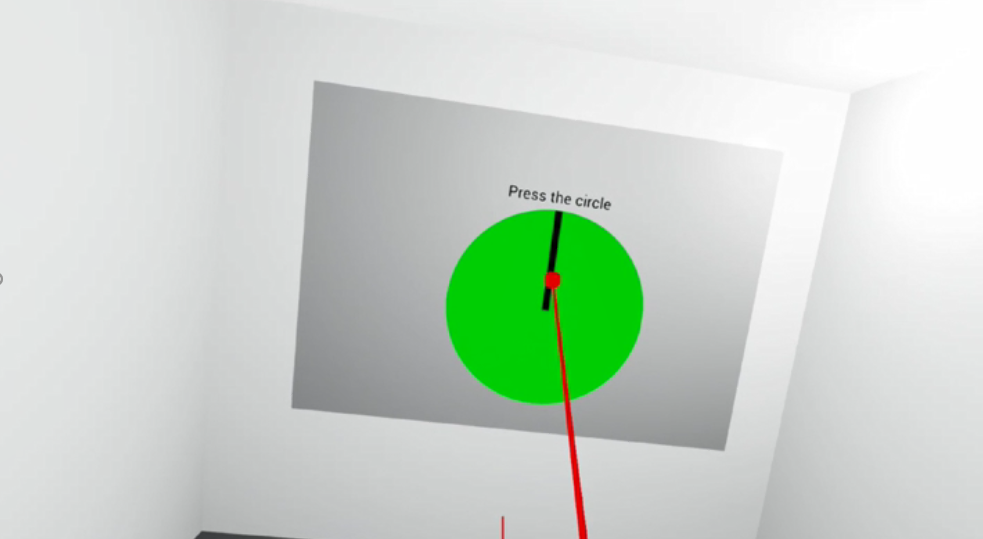
\includegraphics[width=\textwidth]{Images/Boredom.png} 
\caption{ Bild des Langeweile-Szenarios in VR. }
\label{fig:boredom4} 
\end{figure}

